\documentclass[12pt]{article}
\usepackage{graphicx}
\usepackage{amsmath}

\begin{document}
CSCI-4100 Assignment 11\\
1. K-NN Rule\\
The best k according to CV is 12, with $E_{CV}=0.01667$, $E_{in}=0.01333$ and $E_{test}=0.01378$\\
CV error vs K plot:\\
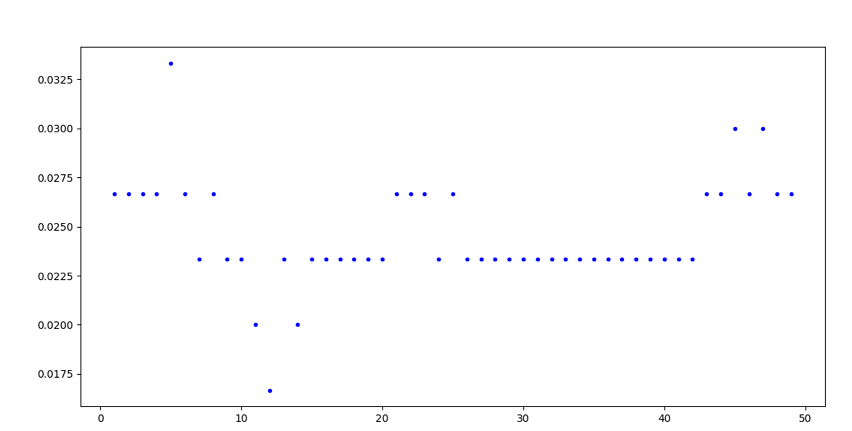
\includegraphics[scale=0.6]{images/knn_ecv_plot}\\
Decision Boundary:\\
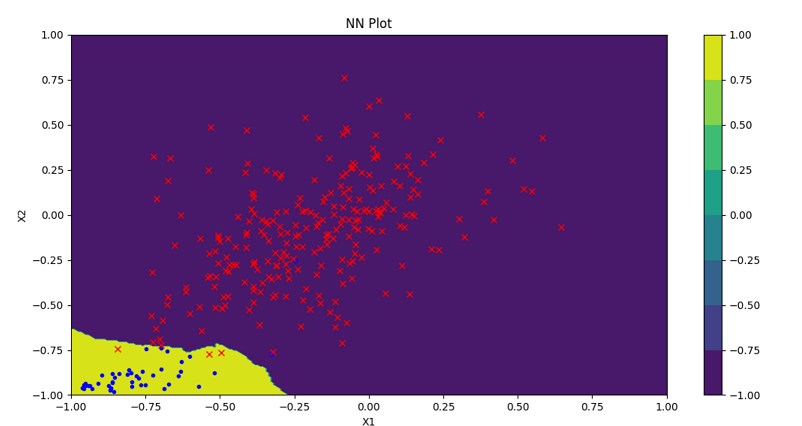
\includegraphics[scale=0.6]{images/knn_decision_boundary}\\\\\\\\\\
2. RBF Rule\\
The best k according to CV is 16, with $E_{CV}=0.06394$, $E_{in}=0.01000$ and $E_{test}=0.01289$\\
CV error vs K plot:\\
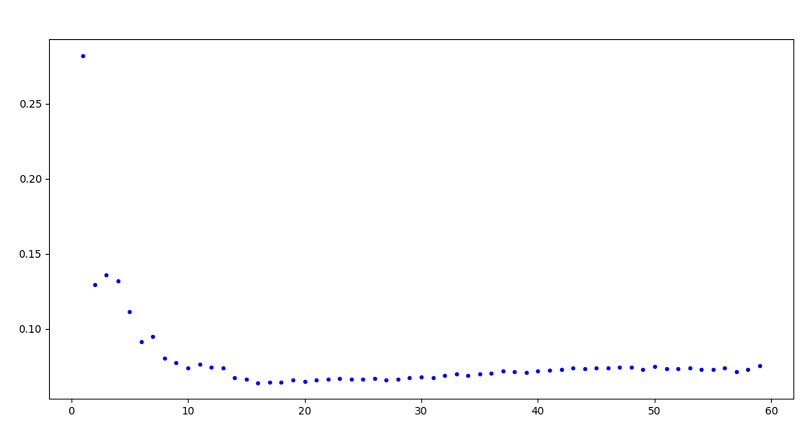
\includegraphics[scale=0.6]{images/rbf_ecv_plot}\\
Decision Boundary:\\
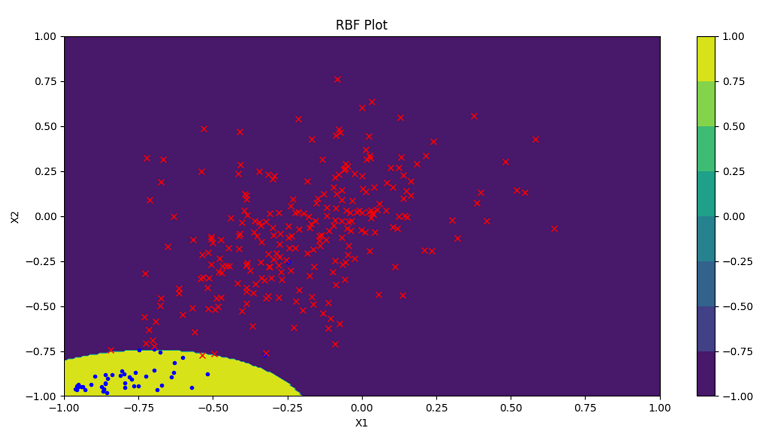
\includegraphics[scale=0.6]{images/rbf_decision_boundary}\\\\
3. Learning Model Comparison
Since the data of homework 9 is not saved, the linear model is run on current set of data points along with KNN and RBF. The result is as following.\\
Decision boundary drawn with training data:\\
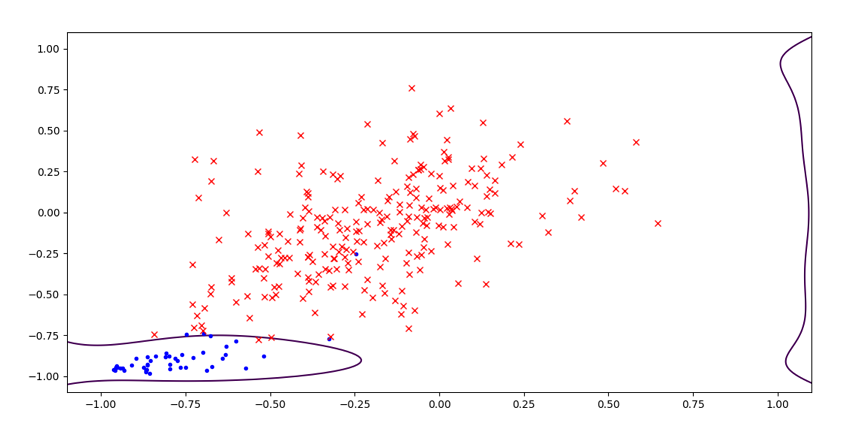
\includegraphics[scale=0.6]{images/linear_train}\\
Same decision boundary drawn with testing data:\\
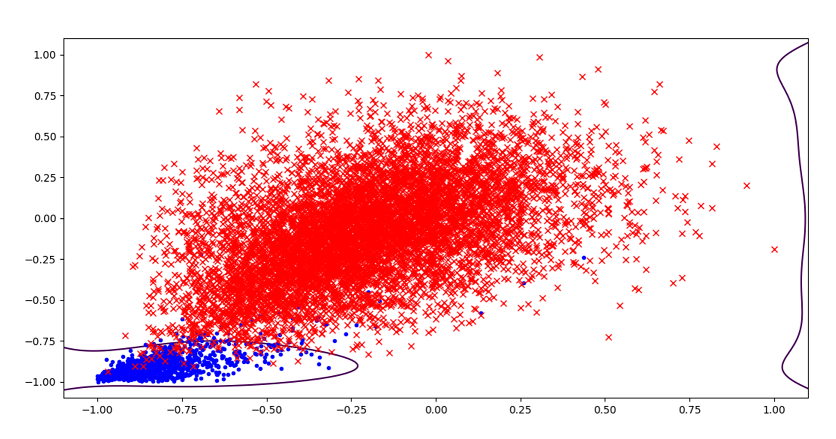
\includegraphics[scale=0.6]{images/linear_test}\\
The best performance is when $\lambda=1.99$ at which $E_{CV}=0.05832$ and $E_{test}=0.01345$\\\\
Here are the test error of all three models:\\
K-NN: $E_{test}=0.01378$\\
RBF: $E_{test}=0.01289$\\
Linear Model: $E_{test}=0.01345$\\\\
All three models have relatively the same performance. One reason that K-NN has slightly higher error is probably because it produces complex hypothesis (its hypotheses set is more complex than the linear model or RBF) and therefore is affected by noise more compare to RBF and the linear model. This can be observed from the decision boundary images, that the boundary of K-NN is less smooth than those of linear model and RBF. \\\\
The fact that RBF performs better that the linear model is probably because the parametric RBF model is actually a linear model with an adaptable linear transform, which provides higher flexibility than regularized linear model. \\

\end{document}












